\documentclass[10pt,a4paper,openany,twoside]{book}
\input{setup/package.tex}   %引用宏包所在位置
\input{setup/format.tex}    %格式所在位置
\begin{document}
%\pagenumbering{Roman}    %Roman字体书写页码
%---------------------------------------------------封面等-----------------------
\include{preface/cover}                         %封面
\include{preface/intro}                          %简介
%\include{preface/intro2}                        %序
\include{preface/preface}                   	    %前言
\include{preface/preface2}                     %前言
\include{preface/preface3}
\include{appendix/acknowledgements}
%\include{preface/c_abstract}             %中文摘要
%\include{preface/e_abstract}             %英文摘要
%-------------------------------------目录部分------------------------------------------
\setcounter{page}{1}   %重新开始页码
\renewcommand\contentsname{目\qquad 录}
%-------------------下面三行去掉了目录首页页码---------------------
\makeatletter
\let\ps@plain\ps@empty
\makeatother
%-------------------------------------------------------------------------
\tableofcontents                                    %目录
%\addtocontents{toc}{\protect\begin{multicols}{2}}       %目录分两栏开始
\mainmatter    %前言和目录页码结束,正文重新开始设置页码
%-----------------------------------------正文开始------------------------------
\include{book/chap1}       %第一章
\include{book/chap2}       %第二章
\chapter{关于虚拟化的一段对话}
\thispagestyle{empty}

\textbf{教授:}首先我们来看操作系统三条简洁之道的第一个: 虚拟化。\newline
\textbf{学生:}但是什么是虚拟化呢? 尊敬的教授。\newline
\textbf{教授:}假设我们有一个桃子。\newline
\textbf{学生:}一个桃子?(怀疑)\newline
\textbf{教授:}是的, 一个桃子。让我们把它叫做实物桃。 但是我们有许多食客想吃这个桃子。我们想向每个食客展示这就是他们的自己的桃子, 这样他们才会高兴, 我们把这个桃子叫做虚拟桃。我们用某种方法让一个实物桃变成若干个虚拟桃。重要的是: 在这种错觉中, 看起来就好像每个人都有一个实物桃, 尽管并不是这样。\newline
\textbf{学生:}所以其实你在分享桃子,但你压根不知道?\newline
\textbf{教授:}是的!\newline
\textbf{学生:}但是这样还是只会有一颗实物桃子。\newline
\textbf{教授:}对的。所以...?\newline
\textbf{学生:}Emmm, 如果我和别人分享桃子,我想我会发现的。\newline
\textbf{教授:}没错!但是大部分时间他们会打盹或在做一些其他事情,这样,我们就可以把桃拿走然后给其他人一会, 这样我们就创造出一种每个人都有一个桃的幻觉\newline
\textbf{学生:}听起来像是个糟糕的竞选口号。你说的是有关计算机的,对吧教授?\newline
\textbf{教授:}噢,你希望有一个更切实的例子。好主意!让我们以最基本的资源:CPU为例。虚拟化所做的就是用这单个CPU,让系统上运行的应用程序看起来有许多虚拟CPU。这样,每个应用程序都认为有属于自己的CPU可以使用,尽管只有一个物理CPU,因此操作系统就创造了一个美丽的幻觉:它虚拟化了CPU。\newline
\textbf{学生:}哇!这听起来就像是魔术,快告诉我更多,它是如何做到的。\newline
\textbf{教授:}听起来你们准备好开始了。\newline
\textbf{学生:}是的!好吧,有一点我必须承认,我有点担心你又开始讨论桃子\newline
\textbf{教授:}别担心;我甚至压根不喜欢桃子,So,我们开始吧...\newline       %第三章
\chapter{抽象:进程}
\thispagestyle{empty}

%\section{引言}
在本章中,我们将讨论操作系统所提供的最基本的抽象之一:\textbf{进程}。进程的非正式定义很简单:进程就是一个\textbf{运行程序}[V+65,BH70]。这个程序本身是没有生命的,它只是磁盘中的一堆程序指令(也许还有一些静态数据),等待被执行。而操作系统所做的就是接收这些指令和数据并且让它们运行起来。

事实证明,人们通常希望能同时运行多个程序,举个例子,想象你有一台笔记本或者台式电脑,上面可能同时运行着Web浏览器,邮件客户端,游戏,音乐播放器等等。事实上,一个典型的操作系统(如windows)上可能同时运行着几十个甚至上百个进程。这样可以让操作系统更加易于使用,人们也永远不需要去关心CPU是否可用;
\begin{tcolorbox}[colframe=grey,colback= grey,arc=0pt,left=6pt,right=6pt,top=6pt,bottom=6pt,boxsep=0pt]
\begin{center}
问题的关键\\
如何提供有许多CPU的幻觉
\end{center}
尽管只有几个物理CPU可用,操作系统该如何提供自己有许多CPU的幻觉。
\end{tcolorbox}
操作系统通过\textbf{虚拟化}CPU来制造这种幻觉。运行一个进程,然后停下,接着去运行另外一个,循环往复下去,这样操作系统就可以提供这种有许多CPU的幻觉, 然而实际上只会有一个或者几个物理CPU,这种技术叫做\textbf{时间共享}(CPU时间片技术),这允许用户想运行多少进程就运行多少进程;不过有个潜在的成本就是性能,所以如果CPU必须共享的话,那么每个进程都会运行地相对慢一些。

为了更好地实现CPU的虚拟化, 操作系统需要一些底层的机器指令和一些高级的算法,我们把这叫做机制, 机制包含的底层方法或协议是实现功能的一个必须部分。比如,我们接下来就要学习如何去实现\textbf{上下文切换},
\begin{tcolorbox}[colframe=grey,colback= grey,arc=0pt,left=6pt,right=6pt,top=6pt,bottom=6pt,boxsep=0pt]
  \begin{center}
  时间共享和空间共享\\
  \end{center}
  \textbf{时间共享}是操作系统共享资源的一种基础技术,该技术允许资源被一个实体占用一段时间,然后被另一个实体占用一段时间,循环往复,这些资源(CPU或是网络链路)可以被许多实体所共享。与时间共享对应的是\textbf{空间共享},在空间共享中,资源会被那些想要使用它的实体分割成许多部分,比如,磁盘就是一种空间共享的资源,一旦一个磁盘块被分配给一个文件,那么在用户删除它之前,这个磁盘块通常不会再被分配给其他文件。
  \end{tcolorbox}
即给予操作系统去中断程序运行从而运行另一个程序的能力,这种时间共享机制(分时机制)被所有的现代操作系统所采用。

在这些机制的基础上,操作系统中的还存在一些以策略的形式存在的智能。策略是在操作系统中进行某种决策的算法。例如,给定一些可能在CPU上运行的程序,操作系统应该运行哪个程序?操作系统中的调度策略将作出此决定,可能会依照一些系统历史信息(例如,哪个程序在最后一分钟运行得更多?),负载信息(例如:有什么类型的程序运行了)和性能指标(例如:系统优化交互性能或是吞吐量)做出决定。
\section{抽象:进程}
操作系统对运行程序所提供的抽象是一种叫做\textbf{进程}的东西,就像之前说的,一个进程就是一个的运行程序,在任何时候,我们都可以通过盘点它在执行过程中访问或影响到的系统的不同部分来总结一个进程。

为了理解进程的构成,我们必须了解他的机器状态:程序在运行时可以读写什么。在任何时候,机器的哪些部分对这个程序的执行很重要?

进程的机器状态的一个明显组成部分就是内存。指令位于内存中;正在运行的程序所读写的数据也位于内存中。因此,进程可以寻址的内存(称为\textbf{地址空间})是进程的一部分。

此外,进程的机器状态的一部分是寄存器;许多指令显式地读取或更新寄存器,因此显然它们对进程的执行很重要。

请注意, 有一些特殊的寄存器构成了机器状态的一部分。例如,\textbf{程序计数器}(PC)告诉我们当前在执行程序的哪条指令;类似的,堆栈指针和相关的帧指针用于管理堆栈中的函数参数, 局部变量和返回地址。

\begin{tcolorbox}[colframe=grey,colback= grey,arc=0pt,left=6pt,right=6pt,top=6pt,bottom=6pt,boxsep=0pt]
  \begin{center}
  单独的策略和机制\\
  \end{center}
  在许多操作系统中,一个共同的设计范式是从低级机制中分离高级策略[L+75]。您可以将机制看作是对如何解决系统的问题提供的答案;例如,操作系统如何执行上下文切换?而策略可以看作是为哪个系统问题提供方案;例如,操作系统现在应该运行哪个进程?将两者分开,可以很容易地改变策略,而不必重新考虑机制,因此这是一种\textbf{模块化}形式,这是一种通用的软件设计原则。
  \end{tcolorbox}
最后,程序也经常访问持久存储设备。这样的I/O信息可能包括当前进程打开的文件列表。

\section{进程API}
尽管我们将有关进程实际的API的讨论放到下一章,在这,我们首先给出一些关于操作系统接口所必须了解的一些概念,这些API以某种可用的形式出现在任何现代操作系统中。

\begin{itemize}
  \item \textbf{Create}:操作系统必须包含一些创造进程的方法,当您在shell中输入命令时,或者双击应用图标时,会调用操作系统创建一个新的进程去运行您指定的程序。
  \item \textbf{Destroy}:因为已经有一个创建进程的接口,所以操作系统还需要一个强制销毁进程的接口,当然,许多进程会运行直到它运行结束时自动退出,当它们不自动退出时,用户也许希望直接杀死进程,所以一个用来销毁进程的接口是十分有用的。
  \item \textbf{wait}:有时,用等待的方式让进程停止运行是很有用的,因此,操作系统通常会提供等待的接口。
  \item \textbf{Miscellaneous Control}:除了杀死或是等待(挂起)进程,通常可能还有其他的控制,例如。大部分操作系统提供一些方法去挂起进程(让进程停止运行一会),然后恢复进程(让进程继续运行);
  \item \textbf{Status}:通常有一些接口去获得一些关于进程的状态信息,比如它运行了多久,或是它现在的状态码。
  \end{itemize}
  \begin{figure}[h]
  \centering
  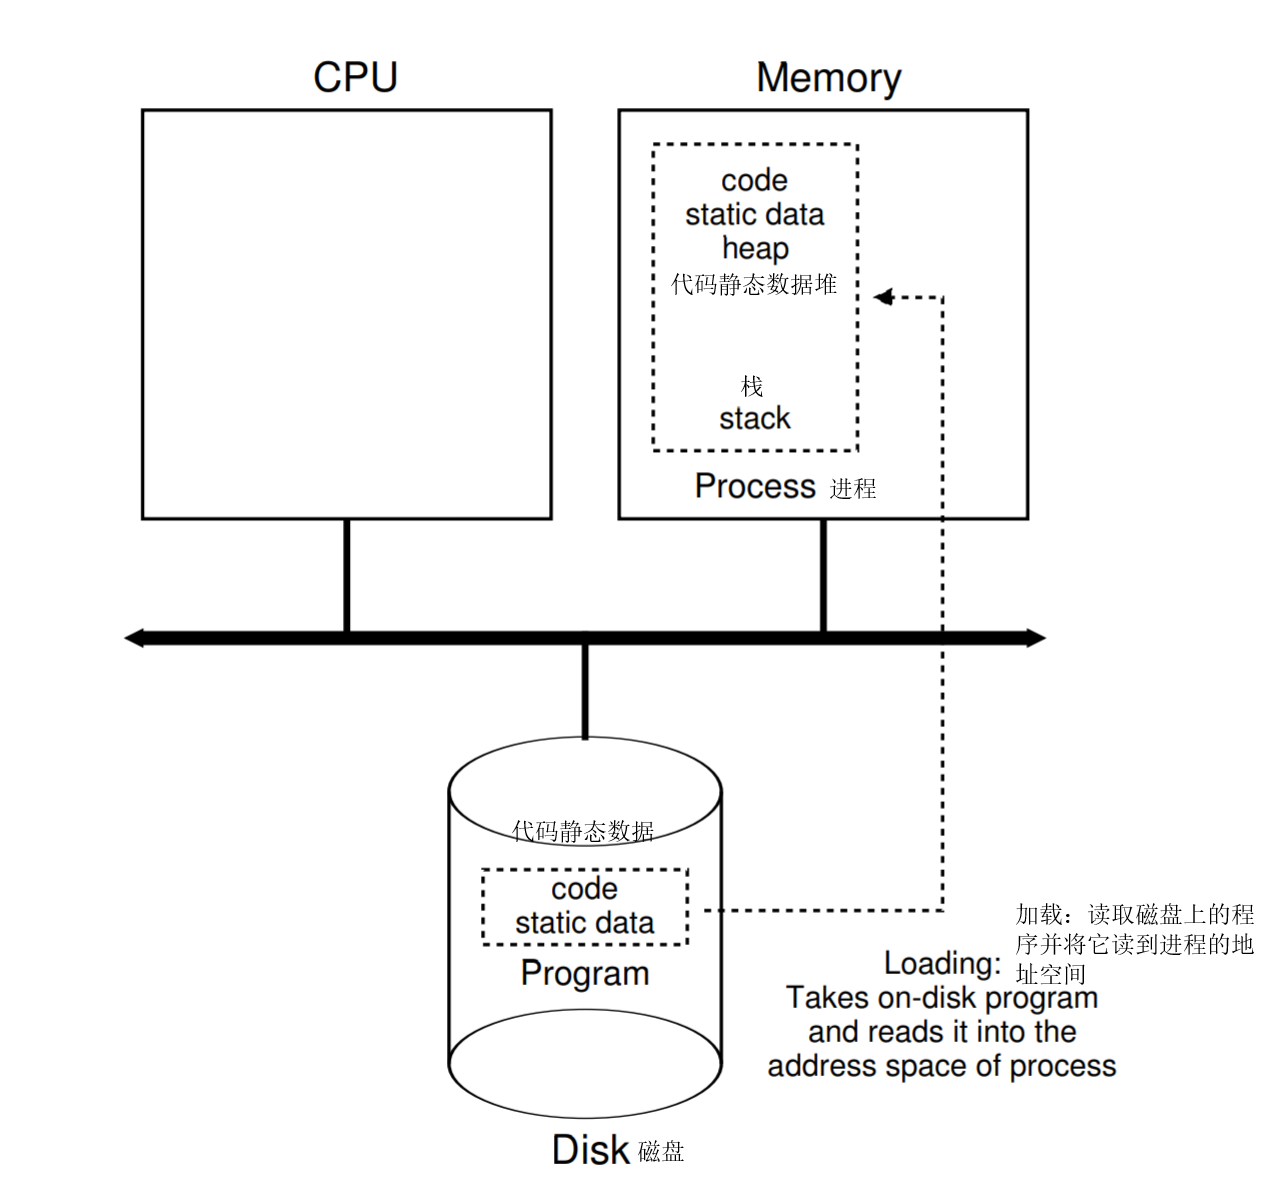
\includegraphics[height=0.5\textwidth]{fig/figure-4-1.png}
  \caption{加载:从程序到进程} \label{fig:figure-4-1}
  \end{figure}   
\section{进程创建:一点小细节}
我们需要揭开的一个谜团是:程序如何转化为进程,具体来说,操作系统是如何启动程序并且运行起来的,进程的创建是如何工作的。

操作系统想要运行程序第一件要做的事情就是将代码和所有的静态数据加载进内存中的进程的地址空间。最初程序是存放在\textbf{磁盘}上(在某些现代系统中,可能是\textbf{SSD})的\textbf{可执行文件},因此,将程序和静态数据加载到内存中的过程要求操作系统从磁盘读取这些字节并将它们放在内存中(如图4.1所示)。

在早期(或简单)的操作系统中, 加载过程是立即完成的,即在程序运行前一次性完成;而现代操作系统是\textbf{延迟加载}的,也就是说在程序执行过程中需要时才会去加载代码或是数据,要真正理解如何延迟加载代码和数据,您必须了解\textbf{分页}和\textbf{交换}机制,这是我们之后讲解内存虚拟化是所讨论的。现在只要记住,在运行任何程序之前,操作系统显然必须做一些工作才能将重要的程序从磁盘转移到内存中。

一旦代码和静态数据加载到内存中,操作系统在进程运行前还会做点小事情。必须为程序的\textbf{运行时堆栈}(或仅仅是堆栈)分配一些内存。您可能已经知道,C程序将堆栈用于局部变量,函数参数和返回地址;操作系统会分配内存并将其中一部分分配给进程,可能还会使用一些参数初始化堆栈;特别的,它会填充main()函数的参数,即argc和argv数组。

操作系统可能还会为程序的\textbf{堆}分配一些内存,在C程序中,堆是用于显式请求的动态分配的数据;程序通过调用malloc()请求这样的空间,并通过调用free()显式地释放它。堆常用于像是链表,哈希表,树或是其他有趣的数据结构,堆最初很小,当程序运行时,通过malloc()库API来请求更多的内存,操作系统可能还会参与其中,并为进程分配更多的内存,以此满足程序的需求。

操作系统还会执行一些其他的初始化任务,特别是有关输入/输出(I/O)的。比如,在UNIX系统中,每个进程默认都会有三个打开的\textbf{文件描述符},用于标准输入,输出和错误;这些描述符使程序可以轻松地从终端读取输入,并将输出打印到屏幕上。我们将在本书中第三部分关于\textbf{持久性}的章节中了解更多关于I/O、文件描述符等方面的内容。

通过将代码和静态数据加载到内存中,创建和初始化堆栈,以及执行与I/O设置相关的其他工作,操作系统已经为程序的执行奠定了基础。它还有最后一个任务;在程序入口点启动程序,即main()。通过跳转到main()例程(通过我们下一章会讨论的专门机制),操作系统将CPU控制权转移给新创建的进程,程序便由此开始执行。

\section{进程状态}
现在我们已经大概了解了什么是进程(我们将继续完善这个概念),以及进程是如何创建的(粗略的),现在让我们来讨论关于进程在不同时间段所处的不同\textbf{状态}。在早期的计算机系统[DV66,V65]中出现了这样一种观点,即进程可以处于这些状态之一。在简化视图中,进程可以处于一下三种状态之一:
\begin{itemize}
\item \textbf{运行态}:在运行态下,进程在处理器上运行。这意味着它正在执行指令。
\item \textbf{就绪态}:在就绪态下,进程已准备好运行,但由于某种原因,操作系统选择在此特定时刻不运行它。
\item \textbf{阻塞态}:在阻塞态下,一个进程执行了某种操作,使它在发生其他事件之前不准备运行。常见示例:进程向磁盘发出了I/O请求,它将被阻塞,因此一些其他进程可以使用处理器。
\end{itemize} 

\begin{figure}[h]
\centering
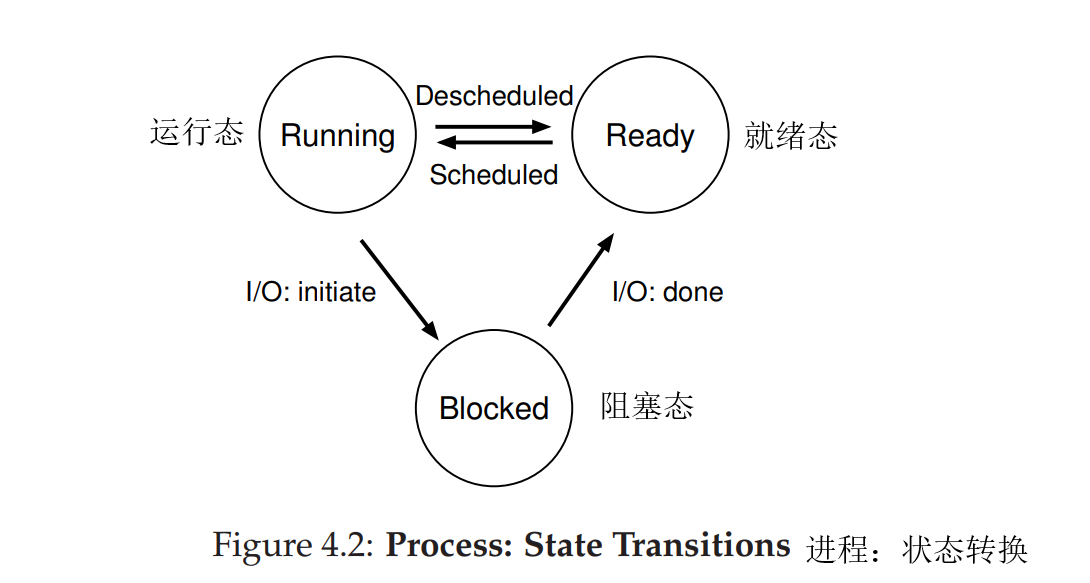
\includegraphics[height=0.5\textwidth]{fig/figure-4-2.png}
\end{figure}   
如果我们将这些状态用图表示,我们将得到图4.2中的图表。正如您在图中所见,进程可以根据操作系统的决定在就绪态和运行态之间切换,从“就绪态”移动到“运行态”意味着进程已经被\textbf{调度执行}从“运行态”移动到“就绪态”因为着进程被\textbf{取消调度}。一旦进程被阻塞(例如,通过启动I/O操作),操作系统将暂停进程,直到某些事情发生(例如I/O操作系完成);此时,进程会再次移动到就绪态(如果操作系统决定继续运行,进程便会立即再次运行)。

让我们看一个例子,来说明两个进程如何通过这些状态进行转换。

首先,假设两个进程正在运行,且每个进程只使用CPU(它们不执行I/O)。在本例中,每个进程的状态跟踪可能如下所示(图4.3)。
\clearpage
\begin{figure}[h]
\centering
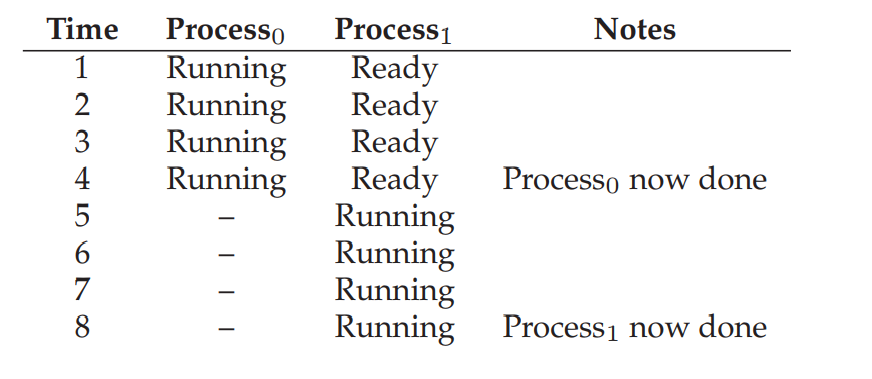
\includegraphics[height=0.3\textwidth]{fig/figure-4-3.png}
\caption{进程状态追踪:CPU} \label{fig:figure-4-3}
\end{figure}
在下个示例中,第一个进程在运行一段时间后发出I/O。此时,进程被阻塞,给另一个进程一个运行的机会。图4.4显示了该场景的跟踪。
\begin{figure}[h]
\centering
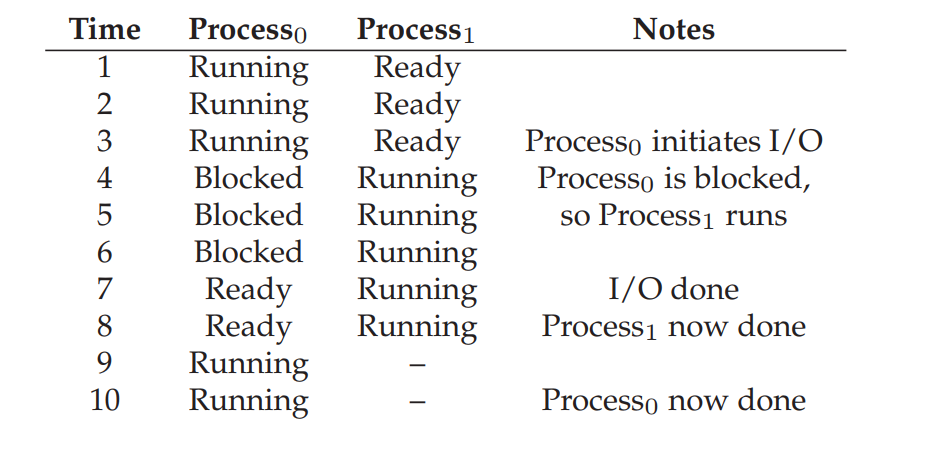
\includegraphics[height=0.3\textwidth]{fig/figure-4-4.png}
\caption{进程状态追踪:CPU和I/O} \label{fig:figure-4-4}
\end{figure}
	
更具体地说,Process 0发出一个I/O请求然后被阻塞,等待I/O完成;进程被阻塞,例如,当从磁盘读取或从网络等待数据包时。操作系统发现Process 0不使用CPU,并开始运行Process 1。当Process 1运行时,I/O完成,将Process 0移回就绪状态。最后,process 1完成,Process 0运行,然后完成。

请注意,即使在这个简单的例子中,操作系统也必须做出许多决定。首先,当进程0发出I/O请求时,系统必须执行进程1,这样做可以保持CPU处于繁忙状态从而提高资源利用率。其次,当I/O完成时,系统会决定不切换回进程0;目前还不清楚这是否是一个好决定。你认为如何?这些类型的决策是由操作系统调度程序做出的,我们将在以后讨论几个章节。

\section{数据结构}
操作系统是一个程序,和任何程序一样,它有一些关键的数据结构来跟踪各种相关的信息。例如,要跟踪每个进程的状态,操作系统可能会为所有已准备就绪的进程放入某种进程列表,并保留一些其他信息来跟踪当前正在运行的进程。操作系统还必须以某种方式跟踪被阻塞的进程;当I/O事件完成时,操作系统应确保唤醒正确的阻塞进程并使其能够再次运行。

图4.5显示了操作系统需要跟踪xv6内核中每个进程的信息类型[CK 08]。类似的数据结构存在于“真实”操作系统中,如Linux、MacOSX或Windows;你可以去查看它们,看看它们有多复杂

从图中,您可以看到操作系统跟踪的有关进程的一些重要信息。对于已停止的进程,寄存器上下文将保存其寄存器的内容。当进程停止时,它的寄存器内存将会被保存到特定的内存位置;通过还原这些寄存器(即将它们的值放回实际的物理寄存器中),OS可以继续运行该进程。我们将在以后的章节中更多地了解这种称为上下文切换的技术。

\begin{lstlisting}
    // the registers xv6 will save and restore
    // to stop and subsequently restart a process
    struct context {
    int eip;
    int esp;
    int ebx;
    int ecx;
    int edx;
    int esi;
    int edi;
    int ebp;
    };
    // the different states a process can be in
    enum proc_state { UNUSED, EMBRYO, SLEEPING,
    RUNNABLE, RUNNING, ZOMBIE };
    // the information xv6 tracks about each process
    // including its register context and state
    struct proc {
    char *mem; // Start of process memory
    uint sz; // Size of process memory
    char *kstack; // Bottom of kernel stack
    // for this process
    enum proc_state state; // Process state
    int pid; // Process ID
    struct proc *parent; // Parent process
    void *chan; // If non-zero, sleeping on chan
    int killed; // If non-zero, have been killed
    struct file *ofile[NOFILE]; // Open files
    struct inode *cwd; // Current directory
    struct context context; // Switch here to run process
    struct trapframe *tf; // Trap frame for the
    // current interrupt
    };
\end{lstlisting}
                图 4.5:xv6 数据结构

从图中还可以看到,除了运行态、就绪态和阻塞态之外,进程还可以处于其他一些状态。有时候,系统会有一个初始状态,当它被创建时,进程就在这个状态中。此外,进程可能处于退出但尚未清理的最后状态(在基于UNIX的系统中,这称为僵尸状态1)。这种最终状态非常有用,因为它允许其他进程(通常是创建进程的父进程)检查进程的返回代码,并查看刚刚完成的进程是否成功执行(通常,程序在基于UNIX的系统中成功完成任务时返回零,否则返回非零)。完成后,父进程将进行最后一次调用(例如,等待(),等待子进程的完成,并向操作系统指示它可以清理任何引用到已灭绝进程的相关数据结构。

\begin{tcolorbox}[colframe=grey,colback= grey,arc=0pt,left=6pt,right=6pt,top=6pt,bottom=6pt,boxsep=0pt]
\begin{center}
旁白:数据结构-进程列表\\
\end{center}
操作系统中充斥着各种重要的\textbf{数据结构},我们将在旁白中讨论这些结构。\textbf{进程列表}(也称为任务列表)是第一个这样的数据结构。这是一个简单的结构,但是任何能够同时运行多个程序的操作系统都会有类似于这个结构的东西,以便跟踪系统中所有正在运行的程序。有时,人们将存储进程信息的单个结构称为\textbf{进程控制块}(ProcessControlBlock,\textbf{PCB}),这是一种包含每个进程信息的C结构的奇特方法(有时也称为\textbf{进程描述符})。
\end{tcolorbox}

\begin{tcolorbox}[colframe=grey,colback= grey,arc=0pt,left=6pt,right=6pt,top=6pt,bottom=6pt,boxsep=0pt]
\begin{center}
旁白:关键进程管理\\
\end{center}
\begin{itemize}
\item \textbf{进程}是正在运行的程序的主要操作系统抽象。在任何时候,进程都可以用状态来描述:\textbf{地址空间}中的内容、CPU寄存器(包括\textbf{程序计数器}和\textbf{堆栈指针}等)的内容,以及关于I/O的信息(例如可以读取或写入的打开的文件)。
\item \textbf{进程API}可由与进程相关的调用组成。通常,这包括创建、销毁和其他有用的API。
\item 进程存在许多不同的状态,包括运行、就绪和阻塞。不同的事件(例如,调度或去调度,或等待I/O完成)会将进程从这些状态中的一种转换到另一种状态。
\item \textbf{进程列表}包含了系统中所有进程的信息。每个条目都存放在\textbf{过程控制块(PCB)}中,PCB实际上只是一个包含特定进程信息的结构体。
\end{itemize}
\end{tcolorbox}

\section{总结}
我们介绍了操作系统最基本的抽象:进程。它很简单地被看作是一个正在运行的程序。考虑到这一观点,我们现在将继续深入讨论细节:实现进程所需的低级别机制,以及高级策略来智能化地控制进程。通过将机制和策略结合起来,我们将建立对操作系统如何虚拟化CPU的独特理解。

       %第四章
%\include{book/chap5}       %第五章
%\include{book/chap6}       %第六章
%\include{book/chap7}       %第七章
%\include{book/chap8}       %第八章
%\include{book/chap9}       %第九章
\include{book/chap26}
\include{book/chap27}
\chapter{锁}
\thispagestyle{empty}

在并发性简介中,我们看到并发编程的一个基本问题:我们想要原子地执行一些列的指令,但是由于单处理器上中断的存在(或者多处理器上多线程并发执行),所以做不到。本章,我们通过提到过的锁来直接解决这个问题。程序员用锁标注源代码,将这些锁放在临界区的周围,因此确保这样的临界区像单条原子指令一样执行。

\section{基本思想}
作为示例,假设我们的临界区如下面的代码,一个典型的共享变量的更新:
\begin{verbatim}
balance = balance + 1;
\end{verbatim}
当然,也有可能是其他的临界区,比如把一个元素添加到链表中或者其他更复杂的共享数据结构的更新,但是这里我们仅仅用这个简单的例子。为了使用锁,在临界区的周围添加一些代码,如下:
\begin{verbatim}
1 lock_t mutex; // some globally-allocated lock ’mutex’
2 ...
3 lock(&mutex);
4 balance = balance + 1;
5 unlock(&mutex);
\end{verbatim}

锁只是一个变量,因此要使用锁的话,必须先声明一个某种类型的锁变量(比如上面的互斥量)。这个锁变量(简称锁)在任何时刻都持有这个锁的状态。它要么是可用的状态,因此没有线程持有这个锁;要么是已获取状态,因此恰有一个线程持有了这个锁,且可能进入了临界区。我们也可以在这个数据类型里存储一些其他信息,比如哪个线程持有了这个锁,或者等待获取锁的队列,但是这些信息是锁用户不可见的。

lock()和unlock()函数的语义很简单。调用函数lock()尝试获取这个锁;如果没有其他线程持有这个锁,这个线程就会获得这个锁并进入临界区;那么这个线程现在就是这个锁的拥有者。如果这时有其他线程对相同的锁变量(本例中的mutex)调用lock()函数,直到它持有这个锁之后才会返回;通过这种方式,就可以防止其他线程在第一个持有锁的线程进入临界区的时候也进入临界区。

一旦锁的拥有者调用了unlock(),锁就会又处于可获取状态(空闲)。如果没有其他线程等待这个锁(比如没有其他线程调用了lock()且阻塞在那里),那这个锁的状态就简单的转换称空闲态。如果有多个等待着的线程(阻塞在lock()函数), 其中一个线程会注意到(或者被通知)锁的状态变化,然后获得锁并进入临界区。

锁为程序员提供了最起码的调度控制。一般讲,我将线程视作由程序员创建但由操作系统调度的实体,不管操作系统选择以何种方式实现。锁将一部分线程调度控制权交还给了程序员;通过在临界区周围放置锁,程序员可以保证不会超过一个线程能进入该临界区。因此,锁将传统操作系统调度的混乱转变得更加可控了。


\section{线程锁}
POSIX库使用的锁的名字叫做mutex,因为它用于在线程间提供互斥量( mutual exclusion),例如,如果一个线程已经进入临界区了,这个线程就会排斥其他线程进来,直到自己执行完临界区的代码。因此,当你看到下面的POSIX线程代码时,你应该能够理解他实际上做的就是上面说的那些(还是使用检测了lock和unlock错误的封装函数):
\begin{verbatim}
pthread_mutex_t lock = PTHREAD_MUTEX_INITIALIZER;

Pthread_mutex_lock(&lock); // wrapper for pthread_mutex_lock()
balance = balance + 1;
Pthread_mutex_unlock(&lock);
\end{verbatim}

也许你还注意到POSIX版本的锁会想lock和unlock传一个变量,是因为我们可能要使用不同的锁来保护不同的变量。这样做可以提高并发性:用不同的锁保护不通的数据和数据结构,这就允许更多的线程马上进入锁住的代码(细粒度的方式),而不是一个任何时候任何临界区都可用的大锁(粗粒度的锁策略)。


\section{构造锁}
到现在为止,从程序员的角度,你应该对锁是如何工作的有了一些理解。但是我们如何构造一个锁呢?硬件需要提供什么支持呢?操作系统又需要支持什么呢?这些问题就是本章剩下的内容要讲的。

\begin{tcolorbox}[colframe=grey,colback= grey,arc=0pt,left=6pt,right=6pt,top=6pt,bottom=6pt,boxsep=0pt]
\begin{center}Crux:如何构造锁\end{center}
我们如何构造一个高效的锁?高效的锁以低开销提供了互斥量,同时也获得了一些其他性质,我们将在后面讨论。硬件需要提供什么支持呢?操作系统需要提供什么支持呢?
\end{tcolorbox}

要构造一个可用的锁,需要我们的朋友——硬件和操作系统提供一些帮助。多年来,个中计算机体结构的指令集都添加了许多不同的硬件原语;虽然我们不需要学习这些指令是如何实现的(毕竟这是计算机体系结构课上的话题),但是我们还是要学习如何使用这些指令来构造一个像锁一样的互斥量原语。我们还会研究操作系统是如何参与完成这个工作的,并帮助我们构建一个精密的锁库。


\section{评估锁}
在构造锁之前,我们应该首先要明白我们的目标是什么,并因此问自己如何评价某个特定锁实现的的效率。要评估一个锁是否有用,应该建立一些基础标准。第一点是,锁能够实现基本的任务,即提供互斥量。基本地,这个锁有效么,能够阻止多线程进入同一个临界区么?

第二点是公平。一旦锁空闲了,是否每个竞争该锁的线程都被公平对待?从另一个方式看的话,就是测试更极端的情况:是否有竞争该锁的线程处于饥饿状态而一直得不到锁?

最后一点就是性能,尤其是用锁后的增加的时间开销。这里有几个不同的情况值得考虑一下。一个是没有竞争的情况;当只有一个线程在运行、获取、释放锁,锁开销有多少?另一个是多线程在单CPU上竞争同一个锁的情况,是否需要担心其性能?最后一点,当引入多CPU,各个CPU上的多个线程竞争同一个锁的性能如何?通过对比这些不同的场景,我可以更好的理解使用各种锁技术对性能的影响。

\section{中断控制}
最早的互斥量的一个解决方案是为临界区关中断;这种方法是为单处理器系统设计的。其代码类似于下面:
\begin{verbatim}
void lock() {
     DisableInterrupts();
}
void unlock() {
     EnableInterrupts();
}
\end{verbatim}

假设程序运行在一个单处理器系统上。通过在进入临界区前关中断(用某种特殊的硬件指令),我们可以确保进入了临界区的代码不会被中断,因此就可以好像原子一样的执行。临界区代码执行结束后重新开中断(还是用硬件指令),因此程序就可以像平常一样继续。

这个方法的好处就是简单。你当然不用想破了脑子去弄明白为什么这方法是可行的。没有了中断,线程就可以保证它执行的代码确实会执行,并且不会有其他线程会干扰它。

可是,负面影响有很多。首先,这个方法要求我们允许任何调用线程取执行特权操作(即中断的开和关),而且还要信任这个功能不会被滥用。正如你知的,任何时候我都要信任随意一个程序,很有可能会有麻烦的。麻烦会以多种方式发生:一个贪心的程序可能在一开始的时候调用lock(),因此而独占处理器;更糟糕的,一个不当的或者恶意的程序可能会调用lock()并进入无限循环。在后一种情况下,操作系统不能重新获得系统的控制权,只有一种办法:重启系统。用关中断作为一种通用的同步方案要求对应用程序太多的信任。

第二,这种方法在多处理器上行不通。如果多个线程运行在多个不同的CPU上,每个线程都试图进入相同的临界区,无论中断是否已经关了,线程还可以运行在其他的处理器上,并因此而进入了临界区。由于多处理器现在很普遍了,我们的通用方案必须要比这个方案好。

\begin{tcolorbox}[colframe=grey,colback= grey,arc=0pt,left=6pt,right=6pt,top=6pt,bottom=6pt,boxsep=0pt]
\begin{center}Aside:Dekker和Peterson的算法\end{center}
在二十世纪六十年代,Dijkstra跟自己的朋友们提出了一个并发性问题,而且其中的一位叫做Theodorus Jozef Dekker的数学家提出了一个解决方案[D68],不像我们这个讨论的方案——用特殊的硬件指令,甚至是操作系统的支持,Dekker的算法仅仅使用load和store(假设它们彼此间是原子的,这在早期的硬件确实是的)。

Dekker的方法后来被Peterson改进了[P81]。这次也仅仅只用了load和store,它的思想是确保两个线程从不会同时进入一个临界区。下面是Peterson的算法(对于两个线程);如果能理解的话,可以看看。flag和turn变量用来做什么呢?
\begin{verbatim}
int flag[2];
int turn;
void init() {
     flag[0] = flag[1] = 0; // 1->thread wants to grab lock
     turn = 0; // whose turn? (thread 0 or 1?)
}
void lock() {
     flag[self] = 1; // self: thread ID of caller
     turn = 1 - self; // make it other thread’s turn
     while ((flag[1-self] == 1) && (turn == 1 - self))
          ; // spin-wait
}
void unlock() {
     flag[self] = 0; // simply undo your intent
}
\end{verbatim}

由于某些原因,一段时间内,开发出不用特殊硬件指令的锁成了时尚,给出了很多问题以及相对应的理论类型。当然,当假设存在硬件支持时,就能更加容易地实现它,那么那些理论型的工作就没有任何用处了(确实这样的支持在多处理器的早期就已经有了)。进一步的,跟上面类似的算法在现代硬件上已经行不通了(因为弱内存一致性模型),因此使得他们比之前更加无用了。然而还有更多的研究被淹没在历史的长河里。
\end{tcolorbox}


第三,也许最不重要的,这个方案的效率很低。与普通指令的执行相比,在现代CPU上中断的开关通常会慢一些。

由于这些原因,关中断只能在有限的情况下作为互斥量原语。例如,当操作系统在访问自己的数据结构时,会用中断的开关来保证原子性,至少可以避免发生繁杂的中断处理情况。这种用法是有意义的,因为信任问题是在OS内部,毕竟不管怎样还是会信任自己执行特权操作的。

\section{test-and-set (原子交换)}

由于关中断在多处理器下行不通,那么系统设计这就开始研究为锁提供硬件支持。最早的多处理系统已经有了相应的支持,比如上世纪六十年代早期的Burroughs B5000。目前所有的系统都提供了这种类型的支持,即使是单CPU系统。

要理解的硬件支持最简单的部分就是test-and-set指令,也被称作原子交换。为了理解test-and-set是如何工作的,我们先试着不用它来构造一个简单的锁。在这个失败的尝试中,我们用一个简单的flag变量来表示该锁是否已被持有。

\begin{figure}[h]
\begin{lstlisting}
typedef struct __lock_t { int flag; } lock_t;

void init(lock_t *mutex) {
    // 0 -> lock is available, 1 -> held
    mutex->flag = 0;
}

void lock(lock_t *mutex) {
    while (mutex->flag == 1) // TEST the flag
        ; // spin-wait (do nothing)
    mutex->flag = 1; // now SET it!
}

void unlock(lock_t *mutex) {
    mutex->flag = 0;
}
\end{lstlisting}
\caption{首次尝试:简单的flag标志}
\end{figure}

在第一次尝试中(图28.1),思想很简单:用一个简单的变量来表示是否有线程已经拥有了该锁。第一个进入临界区的线程会调用lock(),lock()会测试flag是否等于1(),然后将flag置为1来表示这个线程已经持有该锁。当临界区代码执行结束,该线程会调用unlock()将flag清除,因此表示该所不再被这个线程持有。

如果在第一个线程在临界区里时,另一个线程恰好也调用了lock(),这个线程就会简单的在while循环里自旋,等待持有该锁的线程调用unlock()清除flag。一旦第一个线程清楚了flag,在等待的线程就会跳出while循环并将flag置为1,然后进入临界区。

可是,这个代码存在两个问题:一个是正确性,另一个是性能。只要你曾经思考过并发编程,那么正确性问题很简单。想象一下这个代码如表28.1那样交替执行(设flag初始值为0)。

\begin{table}[h]
\centering
{\scriptsize
\begin{tabular}{p{4cm} p{4cm}}
\textbf{Thread 1}&\textbf{Thread 2}\\ \midrule[1.1pt]
call lock() & \\
while(flag == 1) & \\
\textbf{interrupt: switch to Thread 2} &  \\
  & call lock() \\
  & while(flag == 1) \\
  & flag =1; \\
  & \textbf{interrupt: switch to Thread 1}  \\
 flag = 1; //set flag to 1(too!) &  \\
\end{tabular}}
\caption{\footnotesize 轨迹:无互斥量}\color{black}\label{tab26-1}
\end{table}

\begin{tcolorbox}[colframe=grey,colback= grey,arc=0pt,left=6pt,right=6pt,top=6pt,bottom=6pt,boxsep=0pt]
\begin{center}Tip:think about concurrency as malicious scheduler (像恶意调度器一样思考并发性)\end{center}
从这个简单的例子中,你也许感觉需要花点时间来理解这个方法的并发执行。你需要做的是,假设你是一个恶意调度器,总是在最不合时宜的时刻中断线程,以破坏他们为构造同步原语而做的微不足道的尝试。好一个奸诈的调度器!尽管恰好是表中的那个中断顺序的概率不大,但是它是可能的,这就是我们需要阐述的——特定的方法是行不通的。怀着恶意的去思考是有用的!(至少有时候是的)
\end{tcolorbox}

正如你在上述例子中看到的,通过不及时的中断,我们可以很容易的就画出两个线程都将flag置为1且都进入了临界区的场景。这种行为就是内行说的”bad”,很明显这次尝试没能够实现最基本的要求:提供互斥量。

关于性能问题,我们会在稍后多讲一些。性能问题其实是线程等待获取已经被持有的锁的方式:它不停的检查flag的值,这个技术称作自旋等待(spin-waiting)。自旋等待为了等其他线程释放锁而浪费时间。这个时间浪费在单处理器上格外的高,等待线程等待的那个线程甚至无法运行(至少在上下文切换前是不能运行的)【此处是否要注一下】!因此,在开发出更有效的解决方案前,我们还是应该考虑一下如何避免这种浪费的方法。


\section{构造一个可行的自旋锁}
尽管上一个示例背后的思想是好的,但不靠硬件的某些支持来实现目标还是不可能。幸运的是,有些系统提供了基于这个思想创建简单的锁的指令。这个强有力的指令在不同的平台有不同的名字,在SPARC上,是load/store无符号字节指令(ldstub),在x86上是原子交换指令(xchg);这些在不同平台上的指令功能都是一样的。他们一般都称作test-and-set。我们将test-and-set指令的行为定义为如下代码片段:
\begin{verbatim}
1 int TestAndSet(int *ptr, int new) {
2      int old = *ptr; // fetch old value at ptr
3      *ptr = new; // store ’new’ into ptr
4      return old; // return the old value
5 }
\end{verbatim}

test-and-set指令行为是这样的,它返回ptr指向的旧值,同时ptr的值更新为new。当然,关键是这一些列的操作是以原子形式执行的。叫作”test and set”的是因为这条指令能够让你”test”旧值(即返回值),同时也将内存值”setting"为新值;故而,这个略有些强大的指令已经足够用来构造自旋锁(spin lock)了,如图28.2所示。

\begin{figure}[h]
\begin{lstlisting}
typedef struct __lock_t {
    int flag;
} lock_t;

void init(lock_t *lock) {
    // 0 indicates that lock is available, 1 that it is held
    lock->flag = 0;
}

void lock(lock_t *lock) {
    while (TestAndSet(&lock->flag, 1) == 1)
        ; // spin-wait (do nothing)
}

void unlock(lock_t *lock) {
    lock->flag = 0;
}
\end{lstlisting}
\caption{用test-and-set构造简单的自旋锁}
\end{figure}

为确保理解了这个锁为什么可行,再来梳理一下。第一个情况,一个线程调用了lock(),并且目前没有其他线程持有这个锁,因此flag此时值为0。当线程调用了TestAndSet(flag,1),这个例程会返回flag的旧值——0;因此测试(testing)flag值的线程不会在while循环中自旋并获得了锁。这个线程并会原子的置(set)flag的值为1。至此该线程就获得了这个锁。当这个线程执行完临界区的代码,再调用unlock()将flag的值重新置为0。

第二种情况,假设已经有一个线程获得了锁(flag值为1)。这时候,当前线程调用lock()并执行TestAndSet(flag,1)。这次,TestAndSet()会返回旧值,即1(因为此时锁已经被某个线程持有)并且还是将flag置为1。只要锁被其他线程持有,TestAndSet()就会不停地返回1,因此这个线程就会自旋到锁被释放。当flag被某个线程置为0,当前线程就会再次调用TestAndSet(),此时TestAndSet()会返回0,同时将flag置为1而获得该锁并进入临界区。

通过将test(旧值)和set(新值)改成一个原子操作,就可以确保只有一个线程获得这个锁。这就是构造一个可行的互斥量的方法。

你也许也明白了为何这种类型的锁也称作自旋锁。这是要构造的最简单的锁,仅简单的自旋到锁可用为止。为了在单处理器上正确工作,需要有一个可抢占的调度器(比如可通过定时器中断的调度器,以便可以运行其他线程)。不能抢占的话,自旋锁在单处理器上就没有太多的意义了,因为线程在CPU上自旋并不会自己结束。

\section{评估自旋锁}
基于上述的自旋锁,我们可以通过之前提到的指标评估一下它的效率如何。锁最重要的是正确性:是否能够支持互斥量?其答案还是明显是yes:自旋锁一次只允许一个线程进入临界区。因此自旋锁是正确的。

另一个指标是公平性。自旋锁对等待线程的公平性如何呢?能够保证等待线程都会进入临界区么?不幸的是,这个答案不太好:自旋锁没有任何公平性保证。实际上,在竞争中,一个自旋线程会一直自旋下去。自旋锁是不公平的也会导致饥饿。

最后一个指标是性能。使用自旋锁的开销有多大?为了更仔细地分析性能,建议考虑几个不同的情况。第一个,多个线程在单个处理器上竞争锁;第二个,多个线程分散在多处理器上竞争锁。

在单CPU上,对于自旋锁,性能很糟糕;设想这样一种情况,已经持有锁的线程在临界区内是可抢占的。其他每个线程都会尝试获取这个锁,那么调度器可能执行所有其他线程(假设有N-1个线程,不包括当前线程)。这样的话,每个线程在放弃CPU之前都要在一个时间片内自旋,这是对CPU时间的浪费。

然而,在多CPU上,自旋锁的性能还可以(假设线程数与CPU数大致相当)。思路大致是这样的:假设线程A运行在CPU 1上,线程B运行在CPU 2上,同时竞争一个锁。如果线程A(CPU 1)获得了锁,那么线程B试图获取锁的话,就会等待(在CPU 2)。然而,临界区一般会比较短,因此锁会很快就转换称空闲状态,线程B就可以获得锁了。在另一个处理器上自旋等待锁并没有浪费太多的CPU时间,因此效率还可以。


\section{compare-and-swap}
有些系统提供的另一个硬件原语是compare-and-swap指令(SPARC),或者compare-and-exchange(x86)。这条指令的C语言伪代码如图28.3。

\begin{figure}[h]

\begin{lstlisting}
int CompareAndSwap(int *ptr, int expected, int new) {
    int actual = *ptr;
    if (actual == expected)
        *ptr = new;
    return actual;
}
\end{lstlisting}
\caption{Compare-and-swap}
\end{figure}

compare-and-swap的基本思想是检测ptr指定地址的值是否与expected相等;如果相等,就将ptr指向的内存地址更新为new值。如果不等的话,什么都不做。最后都返回actual值,从而可以让调用compare-and-swap指令的代码知道成功与否。

通过compare-and-swap指令,我们可以用与test-and-set指令类似的方法构造一个锁。比如,仅仅将之前的lock()函数替换成这样:

\begin{verbatim}
1 void lock(lock_t *lock) {
2     while (CompareAndSwap(&lock->flag, 0, 1) == 1)
3     ; // spin
4 }
\end{verbatim}

其他的代码与上面的test-and-set例子一样。这段代码的运行过程跟之前的例子很类似;简单地检查flag是否是0,如果是0的话,就原子地的swap新旧值(即将flag置为1)并获得锁。试图获得已经被持有锁的线程会阻塞等待,直到锁被释放。

如果你想看看C可调用的x86版本的compare-and-swap的构造,下面这段代码也许有用[S05]:

\begin{lstlisting}
char CompareAndSwap(int *ptr, int old, int new) {
    unsigned char ret;

    // Note that sete sets a ’byte’ not the word
    __asm__ __volatile__ (
        " lock\n"
        " cmpxchgl %2,%1\n"
        " sete %0\n"
        : "=q" (ret), "=m" (*ptr)
        : "r" (new), "m" (*ptr), "a" (old)
        : "memory");
        return ret;
}
\end{lstlisting}

最后,也许你已经感觉到,compare-and-swap指令比test-and-set要更强大一些。我们将会在后面简要的研究wait-free synchronization[H91]时用到这个指令。然而,如果只是用它构造一个自旋锁的话,这与之前分析的自旋锁没有区别。


\section{load-linked和store-conditional}

有些平台支持一对合同构造临界区的指令。例如,在MIPS架构上[H93],load-linked和store-conditional指令可以联合用来构造锁和其他并发结构。其C伪代码如图28.4所示。Alpha、PowerPC和ARM上都有类似的指令[W09]。

\begin{figure}[h]
\begin{lstlisting}
int LoadLinked(int *ptr) {
    return *ptr;
}

int StoreConditional(int *ptr, int value) {
    if (no one has updated *ptr since the LoadLinked to this address) {
        *ptr = value;
        return 1; // success!
    } else {
        return 0; // failed to update
    }
}
\end{lstlisting}
\caption{Load-linked和Store-conditional}
\end{figure}

load-linked指令的操作与典型的load指令很类似,简单的从内存中取值并将其放入寄存器中。不同之处在于store-conditional,它仅在该地址没有intermittent store发生时成功(并更新相应地址的值,该地址只能是load-linked返回的)。如果成功的话,store-conditional返回1并更新ptr指向的值为value;如果失败的话,不更新ptr指向的值并返回0。

你可以自我挑战一下,试着想想用load-linked和store-conditional指令如何构造一个锁。尝试之后,再看看下面的示例代码提供的一个简单解决方法。试试看,该方法就在图28.5中。

\begin{figure}[ht]
\begin{lstlisting}
void lock(lock_t *lock) {
    while (1) {
        while (LoadLinked(&lock->flag) == 1)
            ; // spin until it’s zero
        if (StoreConditional(&lock->flag, 1) == 1)
            return;  // if set-it-to-1 was a success: all done
                        // otherwise: try it all over again
    }
}

void unlock(lock_t *lock) {
    lock->flag = 0;
}
\end{lstlisting}
\caption{用LL/SC构造锁}
\end{figure}

lock函数才是有趣的部分。首先,某个线程自旋等待flag标志置为0(意味着锁处于空闲态)。一旦锁处于空闲态,这个线程就尝试用store-conditional指令获取锁;如果成功了,那么这个线程就原子地修改flag值为1并进入临界区。

要注意store-conditional指令可能会失败。某个线程调用了lock()并执行了load-linked,得到返回值为0,表示锁处于空闲态。此时,即在执行store-conditional之前,它被中断,另一个线程调用了lock(),也执行了load-linked指令,也得到返回值0。此时,两个线程各自都执行了load-linked指令,并且都将要执行store-conditional指令。这条指令的关键性质就是只有一个线程能成功的更新flag的值为1并获得锁;另一个线程执行store-conditional会失败(因为前一个线程在load-linked和store-conditional之间更新了flag的值)并需要再次尝试获取锁。

\begin{tcolorbox}[colframe=grey,colback= grey,arc=0pt,left=6pt,right=6pt,top=6pt,bottom=6pt,boxsep=0pt]
\begin{center}TIP:更少的代码才是更好的代码(Lauer定律)\end{center}
程序员们在某些事的时候,都倾向于吹嘘自己写了许多代码。这么做从根本上就是错的。然而,需要炫耀的是对于某个任务用了多么少的代码。短小精悍的代码才是更好的选择;这样才有可能更容易的理解并少有bug。当讨论到Pilot操作系统的构建时,Hugh Lauer说道:”如果同一个人有两次机会,那他可以用一半的代码量来构造出一个同样优秀的系统”[L81]。我们称之为Lauer定律,非常值得记住它。所以,下次你在炫耀你在做某项任务时写了多少代码时,请再想想;更好的话,回去重写一遍,把代码写得尽可能的短小精悍。
\end{tcolorbox}

在几年前的课堂上,一位研究生David Cape为那些喜欢用短路布尔条件(short-circuiting boolean conditionals)表达式的同学,提供了一个更简介的形式。如果能够弄明白为什么这两个形式是等价的话,那就看看吧。这确实更短!

\begin{verbatim}
1 void lock(lock_t *lock) {
2     while (LoadLinked(&lock->flag)||!StoreConditional(&lock->flag, 1))
3         ; // spin
4 }
\end{verbatim}

\section{fetch-and-add}
最后一个硬件原语是fetch-and-add指令,它原子地将某一地址的值加1.fetch-and-add指令的C语言伪代码如下所示:

\begin{verbatim}
1 int FetchAndAdd(int *ptr) {
2     int old = *ptr;
3     *ptr = old + 1;
4     return old;
5 }
\end{verbatim}
代码

在下面的例子中,我们将用fetch-and-add指令来构造一个更有意思的排队锁(ticket lock),由Mellor-Crummey和Scott提出[MS91]。lock和unlock代码如图28.6所示。

\begin{figure}[ht]
\begin{lstlisting}
typedef struct __lock_t {
    int ticket;
    int turn;
} lock_t;

void lock_init(lock_t *lock) {
    lock->ticket = 0;
    lock->turn = 0;
}

void lock(lock_t *lock) {
    int myturn = FetchAndAdd(&lock->ticket);
    while (lock->turn != myturn)
        ; // spin
}

void unlock(lock_t *lock) {
    FetchAndAdd(&lock->turn);
}
\end{lstlisting}
\caption{排队锁(Ticket Locks)}
\end{figure}


不像一个单独的值,这个方案里用了ticket和turn变量作为组合来构造锁。其基本操作很简单:当一个线程希望获得锁时,它先对ticket值做一次原子地fetch-and-add操作;此时这个值就作为这个线程的”turn”(myturn)。然后,全局共享变量lock->turn用来决定轮到了哪个线程;当对于某个线程myturn等于turn时,那就轮到了这个线程进入临界区。unlock简单地将turn值加1,由此下一个等待线程(如果存在的话)就可以进入临界区了。

注意这个方法相对于前面的几种方式的一个重要不同:它保证了所有线程的执行。一旦某个线程得到了他自己的ticket值,在将来的某一时刻肯定会被调度执行(一旦前面的那些线程执行完临界区并释放锁)。在先前的方案中,并没有这一保证;比如,某个自旋在test-and-set的线程可能会一直自旋下去,即使其他的线程获得、释放锁。


\section{小结:如此多的自旋}

这些的基于硬件的锁都很简单(只有寥寥数行代码)并且也是可行的(你可以写些代码来证明),这对于任何系统或代码来说都是很好的两个性质。然而,在某些情况下,这些方法都非常的低效。设想,你在单个处理器上运行两个线程。其中一个线程(线程0)正在临界区中,因此锁是被其持有的;它被不幸地中断了。另一个线程(线程1)此时试图获得锁,但是发现它被另一个线程持有了,那么它就开始等啊等啊等,直到最后定时中断到达。线程0再次运行,释放锁,线程1下次运行的时候就不用再等那么久了,它会马上获得锁。因此任何一个发生线程1这种情况的线程,都会浪费一整个时间片做无用功来检测一个根本不会改变的值!如果是N个线程竞争同一个锁的话,情况会更糟糕;N-1个时间片会以类似的方式被浪费——简单的等待单个线程释放锁。那么,我们的下一个问题:

\begin{tcolorbox}[colframe=grey,colback= grey,arc=0pt,left=6pt,right=6pt,top=6pt,bottom=6pt,boxsep=0pt]
\begin{center}Crux:如何避免自旋\end{center}
怎么开发出一个不会浪费时间,不在CPU上无谓自旋的锁?
\end{tcolorbox}

仅有硬件支持不能解决这个问题,还需要操作系统的支持!下面就来弄明白怎么实现这样的锁。

\section{简单方法:放手吧,孩子!}

硬件支持已经让我们走了很远:可行的锁,甚至是获取锁的公平性(ticket lock)。然而,我们还有个问题:在临界区中发生了上下文切换时需要做什么,多个线程开始无休止的自旋等待被中断线程(扔持有锁)在此执行?

第一次尝试一个简单但友好的方法:当线程将要自旋时,换作放弃CPU给其他线程,或者如Al Davis说:”放手吧,孩子!”[D91]。图28.7呈现了这个方法。

\begin{figure}[h]
\begin{lstlisting}
void init() {
    flag = 0;
}

void lock() {
    while (TestAndSet(&flag, 1) == 1)
        yield(); // give up the CPU
}

void unlock() {
    flag = 0;
}
\end{lstlisting}
\caption{Lock with test-and-set and yield}
\end{figure}

这个方法中,假设有一个操作系统原语yield(),可以在需要放弃CPU让其他线程执行时调用它。线程可以处于三个状态(运行、就绪和阻塞)中的一个;yield是一个将调用者从运行态转换称就绪态的简单系统调用,从而推进其他线程执行。因此,yield过程实质上是对自己取消调度(deschedule)。

考虑这么一个简单的例子,有两个线程运行在一个CPU上,我们的这个基于yield的方法就相当的好。如果线程碰巧调用lock(),发现这个锁被其他线程持有了,它就简单地放弃CPU,那么另一个线程就可以运行并完成临界区的任务。在这个简单的例子里,这个yield的方法可以工作的很好。

我们考虑这样的场景,有许多线程(假设100个)不停地竞争同一个锁。此时,如果其中一个线程获得了锁并在释放它之前抢占着;其他99个线程就会各自调用lock(),发现锁不处于空闲态就放弃CPU。假设系统采用某种round-robin调度器,在持有锁的线程在此得到执行前,这99个线程各自都会执行一次run-and-yield流程。尽管比前面讲的自旋方法(会浪费99个时间片来自旋)好,但是这个方法开销还是很大;上下文切换的开销还是很显著的,因此会有大量的浪费。

糟糕的是,我们还是没有解决饥饿的问题。如果其他线程不听的进入、退出临界区,某个线程还是有可能会不停的放弃CPU。显然我们需要一个直接解决这个问题的方法。


\section{队列:休眠而非自旋}

先前的那些方法存在的真正问题是它们将太多的东西交给了运气。由调度器决定下次执行哪个线程;如果调度器做了一个不好的选择,那么该线程要么自旋等待锁(第一种方法),要么立即放弃CPU(第二种方法)。不管哪种方法,都有浪费CPU和引起饥饿的潜在可能性。

因此我们在当前持有者释放了锁之后,必须明确地对哪个线程获得锁采取一些控制。要这么做,需要操作系统提供一些支持,也就是用一个队列来跟踪哪些线程在等待获取这个锁。

简单起见,我们用Solaris提供的两个系统调用:park(),使调用线程进入休眠,unpark(threadID)唤醒threadID指定的某个线程。这两个例程可以联合用来构造一个锁,将试图获取非空闲态锁的线程转换至休眠,当锁被释放后就唤醒这个线程。来看一下图28.8所示的代码以理解使用这个原语的一种方式。


在本例中,将做几个有意思的事情。首先,我们将原来的test-and-set思想和锁等待队列结合来构造一个更高效的锁。第二,我们用一个队列来帮助控制哪个线程下次获得锁,从而避免饥饿。

首先,你也许会注意这些guard是如何使用的,比如锁使用的flag前后的自旋锁和队列操作。这个方法并没有完全避免自旋等待;线程在获取或释放锁时坑你会被中断,从而引发其他线程需要自旋等待这个线程在此执行。然而,自旋花费的时间是相当有限的(仅仅是lock和unlock代码中的几条指令。而不是用户定义的临界区),因此这个方法还是合理的。

其次,你也许注意到lock()中,当某个线程不能获取锁(已被持有)时,会小心的将它添加到队列中(通过调用gettid()获取当前线程的线程ID),将guard置为0然后放弃CPU。读者可能有疑问:如果将guard锁的释放放在park()之后而不是前面,会发生什么呢?提示:something bad。

你也许还注意到一个有趣是事实:当另一个线程被唤醒后,flag的值并没有被置回0。为什么会这样呢?当然这不是一个错误,而是有其必要性的!当一个线程被唤醒,他似乎是从park()中返回的;然而,它此时并没有持有guard,因此不可能将flag置为1。从而,我们只需将锁直接从释放锁的线程传给下一个获取了锁的线程;flag在这之间没有被置为0。

最后,你应该注意到这个解决方案里竞争条件仅仅在lock调用的前面(一直到park())。只需一个错误的实际,某个线程正要执行park(),假定它要休眠到锁不再被持有。此时切换至另一个线程(即持有锁的线程)会导致问题,比如,如果该线程释放了锁。第一个线程紧接着的park()就会永远休眠。这个问题有时被称作wakeup/waiting race;要避免它,还需要一些其他帮助。

Solaris通过添加第三个系统调用:setpark()。通过吊用这个例程,线程就可以表明它将要进入park了。如果刚好发生了中断,且其他线程在真正调用park之前调用了unpark,那么接下来的park就会立即返回而不是休眠。lock()里的代码修改很少:

\begin{verbatim}
1         queue_add(m->q, gettid());
2         setpark(); // new code
3         m->guard = 0;
\end{verbatim}

另一个不同的解决方法,可以将guard传递进内核。这样的话,内核就可以采取预防措施来原子地释放锁并dequeue运行线程。

\begin{lstlisting}
typedef struct __lock_t {
    int flag;
    int guard;
    queue_t *q;
} lock_t;

void lock_init(lock_t *m) {
    m->flag = 0;
    m->guard = 0;
    queue_init(m->q);
}

void lock(lock_t *m) {
    while (TestAndSet(&m->guard, 1) == 1)
        ; //acquire guard lock by spinning
    if (m->flag == 0) {
        m->flag = 1; // lock is acquired
        m->guard = 0;
    } else {
        queue_add(m->q, gettid());
        m->guard = 0;
        park();
    }
}

void unlock(lock_t *m) {
    while (TestAndSet(&m->guard, 1) == 1)
        ; //acquire guard lock by spinning
    if (queue_empty(m->q))
        m->flag = 0; // let go of lock; no one wants it
    else
        unpark(queue_remove(m->q)); // hold lock (for next thread!)
    m->guard = 0;
}
\end{lstlisting}
\begin{figure}[h]
\setlength{\abovecaptionskip}{1pt}
\caption{Lock with Queues、test-and-set、yield and wakeup}
\setlength{\belowcaptionskip}{1pt}
\end{figure}

\section{不同操作系统,不同支持}

目前,就操作系统在线程库中为构造更高效的锁而提供的支持,已经了解过了其中的一种形式。其他的操作系统也提供了类似的支持,细节都不一样。

例如,Linux提供的futex,与Solaris提供的接口类似,但是futex提供了更多内核功能。特别的,每个futex可以与某个特定的物理内存位置关联;与之关联的内存位置是内核队列。线程可以调用futex来休眠或者唤醒。

特别地,还有两个系统调用。futex\_wait(address, expected)调用在address处的值与expected相等时,使调用线程休眠。如果不相等的话,该系统调用会立即返回。futex\_wake(address)调用唤醒等待队列中的某个线程。它们在Linux中的使用方法见图28.9。

\begin{lstlisting}
void mutex_lock (int *mutex) {
    int v;
    /* Bit 31 was clear, we got the mutex (this is the fastpath) */
    if (atomic_bit_test_set (mutex, 31) == 0)
        return;
    atomic_increment (mutex);
    while (1) {
        if (atomic_bit_test_set (mutex, 31) == 0) {
            atomic_decrement (mutex);
            return;
        }
        /* We have to wait now. First make sure the futex value
            we are monitoring is truly negative (i.e. locked). */
        v = *mutex;
        if (v >= 0)
            continue;
        futex_wait (mutex, v);
    }
}

void mutex_unlock (int *mutex) {
    /* Adding 0x80000000 to the counter results in 0 if and only if
        there are not other interested threads */
    if (atomic_add_zero (mutex, 0x80000000))
        return;

    /* There are other threads waiting for this mutex, wake one of them up. */
    futex_wake (mutex);
\end{lstlisting}
\begin{figure}[h]
\setlength{\abovecaptionskip}{1pt}
\caption{基于Linux的Futex锁}
\setlength{\belowcaptionskip}{1pt}
\end{figure}

摘自NPTL库(GNU libc库的一部分)中lowlevellock.h的代码片段[L09]非常有意思。基本地,它用单个integer跟踪锁是否被持有(integer的最高位bit)以及这个锁有多少个等待者(剩余的其他bits)。因此,如果锁是负的,即它被某个线程持有了(因为最高位被置1了,且此位决定integer的符号)。这些代码如此有趣还因为它们展示了在没有竞争的正常情况下如何优化:在仅有一个线程获取、释放锁时,只有很少的开销(lock的atomic bit test-and-set和释放锁的原子加操作)。如果能够弄明白其余这些”real world”锁是如何工作的,那就去看一看吧。


\section{两段(two-phase)锁}

最后一个note:Linux的锁还有一些老方法的味道,老方法已经断断续续的使用了很多年了,最早至少可以追溯到上世纪六十年代的Dahm锁[M82],现在被称作两段锁(two-phase lock)。两段锁实现自旋会很用,特别在锁即将被释放时。在第一阶段,锁自旋一段时间,希望可以获得锁。

然而,如果在第一阶段的自旋中没有获得锁,就进入第二阶段,此阶段调用者进入休眠直到锁变为空闲态后才被唤醒。前面的Linux的锁就是这种锁的一种形式,但是他仅仅自旋一次;这种锁的一个原则就是在调用futex进入休眠前可以在循环中自旋固定次数。

两段锁还是混合(hybrid)方法的另一个实例,这种方法将两个优秀的思想结合以实现一个更好的方法。当然,这种方法是否真的更好还取决于很多其他因素,包括硬件环境、线程数和其他负载细节。通常,构造一个适用于所有可能情况的通用锁,是很具有挑战性的。


\section{小结}
上述的方法讲解了当前真实的锁是如何构造的:一些硬件支持(那些强大的指令)加上一些操作系统支持(Solaris的unpark()原语或者Linux的futex)。当然,各自的细节都不尽相同,实现这些锁的代码都是非常优秀的。如果想要了解更多细节的话,可以去看Solaris或Linux的代码库;它们都非常吸引人[L09,S09]。也可以看看David等人对比现代微架构上各种锁策略的优秀的成果[D+13]。


%\newpage

%参考文献\\







\include{book/chap29}
\include{book/chap30}
\include{book/chap31}
\include{book/chap32}
\include{book/chap33}
\include{book/chap39}
%\addtocounter{chapter}{7}
%-----------------------------------------正文结束------------------------------
\include{book/answer}      %习题答案
%\addtocontents{toc}{\protect\end{multicols}}   %目录分两栏结束
\include{reference/references}                               %参考文献部分
\clearpage
\end{document}



